\chapter{Project Background}
\label{chap:antecedentes}


\drop{T}{his} chapter summarized the background required to accomplish the
GEO-Cloud project. Thus, the study of the state of the art will be done by
focusing in some aspects of cloud computing platforms, federated testbeds,
networking and satellite systems. As a consequence, this section describes the different thematic areas.
The conceptual map showed in Figure~\ref{fig:intr-conceptual-map} shows the
sections and subsections of this chapter. Thereby in the Earth Observation
satellites area, the different concepts for creating and modelling a satellite
for remote sensing are studied together with its data management and orbital
definitions. In high-level languages, some scripting languages are required. In
Networking,the different existing network impairments and the tools required to
measurement are explained. In Federated Infrastructures, the testbeds that
constitute the \emph{Fed4FIRE} insfrastructure are studied. In Graphical User Interfaces, the several
frameworks for developing \acp{GUI} are described. In Databases, the database
management systems are detailed. In distributed systems, the middlewares such as \emph{Hadoop} or
\emph{ZeroC Ice} for developing distributed applications are related. And finally, in
the Software Design, the requirements for building multiplatform code and other
ancillary libraries required by the detailed objectives of GEO-Cloud are explained.

\begin{figure}[!h]
\begin{center}
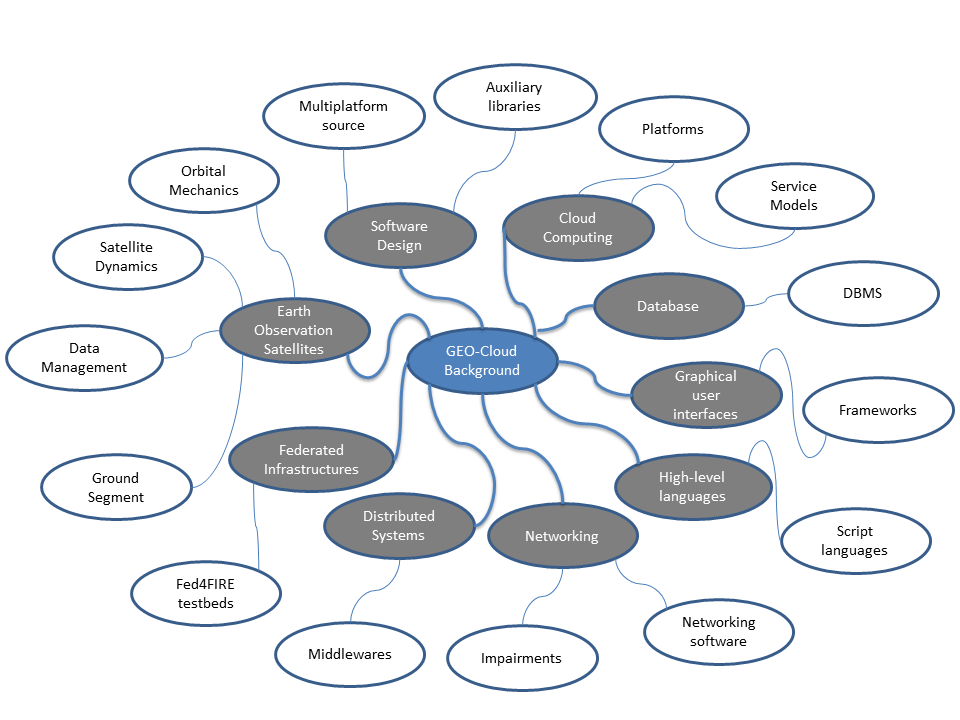
\includegraphics[width=1.0\textwidth]{statement/background-geocloud.png}
\caption{Conceptual map of this chapter.}
\label{fig:intr-conceptual-map}
\end{center}
\end{figure}


\section{Earth Observation Satellites}

In this section, different areas of aeronautics are involved: Orbital
Mechanics defines and calculates the satellite orbits for rounding around
the world;  Spatial Telescopes  contribute with the payload parameters and the
data management processes on the fly, stores and sends the science and ancillary
data from satellites to the Ground Segment.

\subsection{Orbital Mechanics}

This field~\cite{Braeunig2013} studies the motion of the satellite considered as a point with no
mass in space affected by \emph{Newton's Laws of Motion} and \emph{Newton's Law of
Universal Gravitation}.
\emph{The Newton's Law of Universal Gravitation} dictates that \emph{any two bodies in the
universe attract each other with a force that is directly proportional to the
product of their masses and inversely proportional to the square of the distance
between them.}
%~\cite{http://en.wikipedia.org/wiki/Newton\%27s_law_of_universal_gravitation}

\begin{equation}
F~= G~*~{\frac {m_1*m_2}{r^2}}
\end{equation}
where $F$ is the force between the masses, $G$ is the gravitational constant
($6.67~x~10^{-11}~\frac{Nm^2}{kg^2}$), $m_1$ and $m_2$ are the first and second
mass in kilograms respectively
and $r$ is the distance in meters between the centres of the masses.

Orbital Mechanics focuses on the trajectories of the
spacecrafts, manoeuvres for orbital acquisition, orbit maintenance and end of life
disposal.

Spacecrafts motion  is governed by the \emph{Kepler's Laws of Planetary
  Motion}~\cite{Stern2014} which can be derived from \emph{Newton's Laws}. These laws are the following:
\begin{enumerate}
\item The orbit of a planet is an ellipse with the Sun at one of the two foci.
\item A line segment joining a planet and the Sun sweeps out equal areas during
  equal intervals of time.
\item The square of the orbital period of a planet is proportional to the cube
  of the semi-major axis of its orbit.
\end{enumerate}


\subsection{Spatial Telescopes}

The \ac{EO} satellites carry on board telescopes pointing to the Earth in order
to acquire images of its surface. The information can be obtained in several
kinds of spectral bands as visible, near infra-red, thermal, etcetera. This
mission uses visible multispectral telescopes distributed in a constellation of satellites
to obtain a global map in a daily basis. For selecting the telescopes~\cite{Ball2013}, the swath
and the \ac{GSD}
have been analysed. The number of satellites is depends on the width of the
swath and the telescope resolution is required to achieve quality
images for the mission.

Depending on the spectral bands used for imaging, the applications may be
different. For example, scientific applications such as soil categorization,
vegetation analysis oroceanography use hyperspectral imagers, which offers
information about hundreds of bands. Other applications such as traffic monitoring,
urban development and surveillance commonly require multispectral imagers with visible bands.

\subsection{Data Management}

Each satellite of the constellation acquires images which have five spectral
bands into the visible spectrum. When this spectral data is
obtained by telescopes, it is necessary to convert from analogical to digital
data. This process is carried out using 12 bits per pixel to codify the
intensity signal level with a digital value. Then, the digital data is stored and pre-processed on
board.

During the pre-processing activity, some meta-data also known as ancillary
data, is added. The ancillary data enriches the acquired sector of image by adding
some geolocated information and transmission auxiliary meta-data for communication
protocols.

All the pre-processed data is aggregated in the
internal storage for downloading when the satellite comes into a visibility zone
of a ground station. In the very moment that the satellite enters into the footprint of a
ground station, the acquired images are downloaded.

The data download is done by multiplexing the
communication channel within two ways. A section of total bandwidth
is used for downloading the images that are being acquired in real time and the
rest of the bandwidth performs the download of the stored images located in
internal storage units.

\subsection{Ground Segment}

The Ground Segment is composed by the antennas, the control centre and the
infrastructures for processing and distribution of images namely processing
data centre.

The current industries of \ac{EO} imaging perform the processing, storage and distribution on premises. The steps are the following:
\begin{enumerate}
\item First, the antennas receive all the data from the satellites and it is stored.
\item Then, the data centre obtains the images from the ground stations.
\item The data centre starts to process available images.
\item When an image has been processed it is archived and catalogued.
\item Finally, the image can be distributed to end users.
\end{enumerate}

The proposed architecture on-cloud  in this project, reduces the delivery time making shorter the cataloguing and archiving times.

In order to implement the archive and catalogue module in cloud, several
platforms for sharing geospatial data were studied. These software servers are
\emph{GeoServer}\cite{Geoserver2014} and \emph{GeoNetwork}~\cite{Community2014} among others.
\begin{itemize}
%http://geoserver.org/about/
\item \emph{GeoServer:} It is a Java-based software server for cataloguing and
  archiving geospatial images among others functions, that uses \ac{OGC}
  standards and allows users to view geospatial images. By default it offers
  \ac{WFS} services and \ac{WPS}. In GEO-Cloud, the Archive and Catalogue module
  has been implemented using \emph{GeoServer} in assembly with its \ac{CSW}
  extension, because it is flexible, simply,
  multiplatform, open source and it can receive data from other sources. It can
  also be integrated with \emph{GeoNetwork}.
%http://geonetwork-opensource.org/
\item \emph{GeoNetwork:} It is a Java-based and platform independent catalogue application to manage
  geospatial images. It uses \ac{OGC} standards such as \ac{CSW}, \ac{WMS} and \ac
  {WCS} among other interchanges protocols. It catalogues data from sources but
  it does not maintains its data. For this reason \emph{GeoServer} was selected.
\end{itemize}

\section{High-level languages}
\label{sec:high-level-languages}
For the development of the project, \ac{XML}, \ac{JSON}, \emph{Python} and \emph{Bash} languages has
been used. The first, \ac{XML}, has been used for building the configuration file of
the Orchestrator component and to obtain the selected nodes by \emph{JFed}
application. \ac{JSON} was used to create the experiment descriptor for the
\bonfire platform. The source of the
components of the cloud has been developed using \emph{Python} and the interconnections
between modules and others secondary functionalities, in \emph{Bash script}.

\subsection{XML}
\ac{XML}~\cite{St.Laurent1998} is a mark-up language that defines a set of rules for encoding
documents in a format that is both human-readable and machine-readable. Most of
actual software use it for configuring or for updating its configuration on fly.

\subsection{JSON}

\ac{JSON}~\cite{Organization} is a lightweight language for data interchange between applications. The
simplicity of \ac{JSON} results very simple and human-readable way to transmit data
objects consisting of attribute-value pairs. Web applications are using this
language substituting \ac{XML} because parsing and generating \ac{JSON} is more efficient
and quick. The \bonfire interface uses it for creating experiment descriptors
ought to the resources provided by the platform can be translated into objects
and its features.

\subsection{Scripting languages}

The Scripting technics consist of using an interpreted programming language in
order to provide advanced mechanisms to specify the functionalities of an
application. The most important features of a scripting language are that it is not
compiled and it permits effortless development. Furthermore, some interpreted languages
are multiplatform because they do not require the compilation of the source for
running the application in a target platform.


\subsubsection{Python}
%https://www.python.org/
\emph{Python}~\cite{Foundation2014} is an object oriented language, although permits imperative and functional
programming. It does not need to compile the source because it is
interpreted. It permits a flexible development because it is dynamically typed
and multiplatform. With this feature, the software can be
executed in any platform. The current version is 2.7.4 and it offers several
useful and multipourpose libraries such as \emph{Matlib, Pthread, Mysqllib and Pdb}.

\subsubsection{Bash Script}

\emph{Bash}~\cite{Cooper2014} is a command language interpreter for the \ac{GNU}
operative system. \emph{Bash} is fully compatible with other command language
interpreters like \emph{sh} or \emph{ksh}, so the source developed by
\emph{Bash} is portable. The Bash scripts contain
commands  to be executed by the interpreter. It provides a direct line
to communicate with the operative system and makes some functionalities ad-hoc.
The \emph{Bash} language consists of several sentences that the operative system
can to read and translate to play a specific action. All current \emph{Linux} distributions contain a Bash interpreter.

\subsubsection{Ruby}
%https://www.ruby-lang.org/en/
\emph{Ruby}~\cite{Community} is an object-oriented, cross-platform, general-purpose and dynamic
programming language. It was designed and developed by \emph{Yukihiro
  Matsumoto}. This language has a dynamic type influenced by Groovy, Falcon and
other ones. It permits an easy, flexible and agile development.


\subsubsection{Lua}
\emph{Lua} is a lightweight, cross-platform, prototype-based, object-oriented programming
language. It was designed and developed by \emph{Roberto Lerusalimschy}. This
language is influenced by C++, Modula and Scheme among others. It provides
native data structures as tables, records and associative arrays which this
structure perform high throughput~\cite{Organization2014}.


\section{Networking}

For simulating an environment as realisticallyl as possible in GEO-Cloud, the impairments  of the networks between both Ground Stations and Cloud Platform
and between both Cloud Platform and end-users had to be acquired. In addition, features
like the bandwidth is obtained in order to stablish the maximum throughput of
channel over \emph{Virtual Wall}.

There are several simulators that
calculates the value of these network features roughly but the obtained results
may be wrong. Therefore, a sub-experiment explained in
Section~\ref{sec:planetlab} for acquiring these values was implemented.

\subsection{Impairments}

The communication through the Internet is not perfect~\cite{Tanenbaum2003} because there are many
sources or random events that affect traffic packets that are traversing a
different network  at any given moment. This is a main issue to take into
account when modelling a network. The main
impairments of a network are the following:

\begin{itemize}
\item \emph{Packet Loss:} this is the disappearance of a packet that was
  transmitted.
\item \emph{Packet Delay:} also known as ``Latency'' is the amount of time that elapses between the time a
  packet is transmitted to a physical environment until the packet is received by
  the target. This delay is composed by three types of delay times: \emph{Propagation
  delay}, which is the time in which the packet arrives its destination;
  \emph{Routing/Switching} delay, which is the time in which the routers or
  switches  process the packet; and finally the \emph{Queuing} delays, which are
  the time the packet is queued in any intermediate hardware of the entire network.
\item \emph{Jitter:} jitter is a measure of the variation in the packet delay
  experienced by a number of packets.
\item \emph{Packet Duplication:} may occurs when one packet becomes two or more
  identical packets.
\item \emph{Packet Corruption:} it occurs when the payload of the packet (even a bit)
  is damaged but the packet continues to flow towards the destination instead of
  being discarded.
\end{itemize}

In the GEO-Cloud project, the impairments considered are \emph{Packet Loss} and
\emph{Packet Delay}, which permit modelling a simulated and close to reality network.


\subsection{Networking Software}

In the networking subject, there are lots of tools that facilitate the obtantion
of the
features values for the metrics defined in a network.
For measuring the throughput, the bandwidth and the loss-rate the following
tools can be used:

\begin{itemize}
\item \emph{Microsoft's
    NTttcp~\cite{Microsoft2013}:}
  this tool is optimized for Windows environments and it similar to
  \emph{Iperf}. Testing impariments in networks can be done using this tool.
\item \emph{NetCPS:~\cite{Aase1998}} The most basick network testing can be performed to give a
  good baseline of network performance. This tool is optimized for Windows
  enviroments.
\item \emph{Iperf~\cite{Iperf2014}:} the most popular tool to measure maximum \ac{TCP} bandwidth, allowing the
  tuning of various parameters and \ac{UDP} characteristics. \emph{Iperf} reports
  bandwidth, delay, jitter and datagram loss. \emph{JPerf} is a Java-extension for
  providing a graphical user interface.
\item \emph{Uperf~\cite{Microsystems2013}:} is a network
  performance measurement tool that supports the execution of workload profiles. It
  is more complex and complete than \emph{Iperf} or \emph{NetPerf} allowing the user to model
  an application using a very high level language and running this over the
  network. It allows the experimenter to use multiple protocols, by varying message sizes to
  collect statistics.
\item \emph{NetPerf~\cite{Company2012}:} is a benchmark that can be used to measure the performance of many different types of networking. It provides tests for both unidirectional throughput, and end-to-end latency.
\end{itemize}

For measuring the delay time the following tools are depicted:
\begin{itemize}
\item \emph{Ping:} it is the most used tool for testing the reachability of a host on an
  Internet Protocol network and for measuring the round-trip-time for packets sent
  from a source host to a target host. \ac{ICMP} protocol is used for it.
\item \emph{Traceroute:} is a networking tool for displaying the path and
  measuring transit delays of packets across a network over the Internet
  Protocol. This command is available on a number of modern operative systems. By
  default it works in network layer of the \acs{OSI} model, sending \ac{UDP} packets but it can be customized
  for sending \ac{ICMP} packets.
\end{itemize}

\section{Federated Infrastructures}

In this section, some federated infrastructures are described. This
infrastructures are used by experimenters for creating new network topologies,
 distributed applications and new network protocols.

A federated infrastructure is a set of unified and autonomous platforms which
are joined in order to provide interoperability and coordinated
information sharing among individual components.

The federated architecture pattern was first used by the \emph{US Federal CIO} in
1990s. Then other organizations adopted this paradigm for its infrastructure
technologies. Nowadays, this topology is growing up in business where the
technological infrastructure has to be distributed, and using critical information around the world.

The benefits of using this kind of network topology are enumerated as follows:
\begin{itemize}
\item Independence: the components of the federation has its own rules,
  protocols and subcomponents. All of them provide an interface for
  communication between others federation components.
\item For the end-users the federated cloud provides an easily way to host apps
  and the automatically selection of resources from different federated components.
\end{itemize}

There are several federated infrastructures for experimentation. These are known
as ``Federated testbeds''. The most important ones are the following:
\begin{itemize}
%{http://ac.els-cdn.com/S1389128613004507/1-s2.0-S1389128613004507-main.pdf?\_tid=320d2494-118e-11e4-9e39-00000aacb35e\&acdnat=1406026495\_7cd6d5a33b3ddfeaf3aad7216039f876}
\item \emph{GENI\footnote{For more information, see
  \url{http://www.geni.net/}}}: The \emph{Global Environment for Networking Innovation}, is a distributed virtual
laboratory for the future internet sponsored by the \emph{U.S. National Science Foundation} for
experimenting. In this platform developments such as protocol
design and evaluation, distributed services or content management may be carried
out~\cite{Berman2014}.
%~{http://www.cs.cmu.edu/afs/cs/usr/droh/www/papers/opencirrus-ieeecomputer.pdf}
\item \emph{Open
  Cirrus:} The \emph{Open Cirrus} testbed provides a federation in cloud computing for
experimentation. In order to support these experiments, global services were added by
providing distributed common services~\cite{Avetisyan2010}. The experiments that can be carried out
in this testbed are large-scale clustering experiments, machine learning and scientific computing. \emph{Open Cirrus} is composed by 10 sites in North
America, Europe and Asia and the platform has been developed by the
\emph{U.S. National Science Foundation}, \emph{the University of
  Illinois},\emph{ the Karlsruhe Institute of Technology}, \emph{the Infocomm Development Authority of Singapore},\emph{ the
Russian Academy of Sciences}, \emph{the Electronics and Telecommunications Research
Institute of South Korea}, \emph{the Malaysian Institute of Microelectronic
  Systems} and \emph{Carnegie Mellon University}. This project is sponsored by Hewlett-Packard, Intel
and Yahoo!~\footnote{For more information, see \url{http://opencirrus.org}}.

\item \emph{Fed4FIRE:} The \emph{Fed4FIRE} is an Integrating Project under the European
Union's \ac{FP7} addressing the work programme topic Future Internet Research
and Experimentation. The project is performed by a consortium of 29 partners
organisations from 8 countries. The \emph{Fed4FIRE}  proposal consists of the
creation of heterogeneous and federated platform with different kinds of services and applications such
as cloud computing, grid computing, smart cities, wireless networking and
large-scale experiments. The federation is composed by the following testbeds:

\begin{itemize}
\item \emph{Virtual Wall:} for creating network topologies.
\item \emph{PlanetLab Europe:} for experimenting with nodes around the world.
\item \emph{Norbit:} for experimenting with Wi-Fi resources.
\item \emph{w-iLab.t:} this testbed is intended for Wi-Fi and sensor networking experimentation.
\item \emph{NETMODE:} it consists of Wi-Fi nodes connected with some processors
  for networking experimenting.
\item \emph{NITOS:} it is a testbed offered by \emph{NITLab} and consists of wireless
  nodes base on open-source software.
\item \emph{Smart Santander:} this is a large scale smart city deployment in
  Santander city of Spain to experiment Internet of Things.
\item \emph{FuSeCo:} this testbed provides resources to experiment with 2G, 3G
  and 4G technologies.
\item \emph{OFELIA:} for testing and validating research aligned
  with Future Internet Technologies.
\item \emph{KOREN:} it provides programmable virtual network resources with
  necessary bandwith connecting 6 large cities at the speed of 10 Gbps to 20 Gbps.
\item \emph{BonFIRE:} it is a multicloud tesbed for experimenting.
\item \emph{performLTE:} it is a realistic environment for creating experiments
  using the \ac{LTE} technology.
\item \emph{Community-Lab:} it is a distributed infrastructure for researchers
  to experiment with community networks for creating digital and social environments.
\item \emph{UltraAccess:} it provides several Optical network protocols and
  resources to experiment with \ac{QoS} features, traffic engineering and virtual \acp{LAN}.
\end{itemize}
\end{itemize}


In GEO-Cloud project, the testbeds used for implementing are \emph{Virtual
  Wall}, \emph{PlanetLab} and \emph{BonFIRE}. These facilities are explained in the next sections.

\subsection{Fed4FIRE Testbeds}

In the previous section the \emph{Fed4FIRE's testbeds} were numerated. Next, the
facilities used in GEO-Cloud are detailed.

\subsubsection{Virtual Wall}

\vw is an emulation environment for
experimenting with advances networks, distributed software and service
evaluation carried out by the \emph{University of Ghent}. It offers the possibility for experimenters to create any type of
network topology, e.g. emulating a large multi-hop topology, client-server
topologies among others and to check algorithms or protocols for subsequent
marketing.
Two \vw testbeds are available: \vw 1 contains 200 servers: 100
quad-cores and 100 eight-cores; \vw 2 contains 100 dodeca-cores.

All servers have a management interface and five Gigabit Ethernet connections
interconnected all of them by switches. On each of these links, the network
impairments can be configured. There are also some virtual machines for
customising the resources. Finally, the network
impairments are configurable~\cite{Wall2014}.

\subsubsection{PlanetLab Europe}

\pl \emph{Europe} is part of the \pl global system, the world's largest
research networking facility, which gives experimenters access to
Internet-connected Linux virtual machines. About 1000 servers conform \pl
platform located in United States, Europe, Asia and elsewhere as Figure~\ref{fig:intr-planetlab-europe} depicts.
This platform can be used by experimenters in order to develop and to check
distributed systems, network protocols, peer-to-peer systems, network security
and network measurements among others applications~\cite{Europe2014}.

Through \emph{Fed4FIRE}, the experimenters can reserve and deploy some
PlanetLab Europe resources and to experiment with them.

\begin{figure}[!h]
\begin{center}
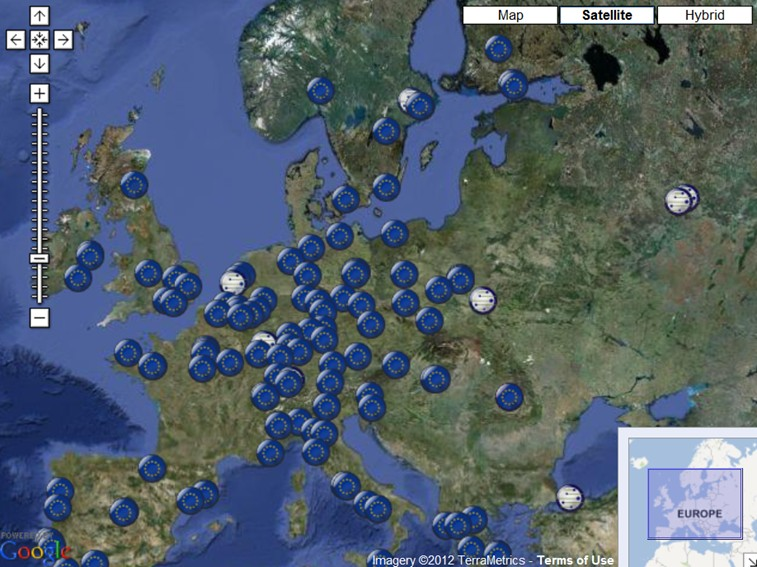
\includegraphics[width=0.65\textwidth]{statement/planetlab-europe.jpg}
\caption{Geographical distribution of PlanetLab Europe.}
\label{fig:intr-planetlab-europe}
\end{center}
\end{figure}

\subsubsection{BonFIRE}

\emph{BonFIRE}~\cite{Hume2012} is a multi-cloud testbed based on an \ac{IaaS}
delivery model with guidelines, policies and best practices for
experimenting. Currently, \bonfire is composed by 7 geographically distributed
testbeds, which offer heterogeneous cloud services, compute resources and
storage resources~\cite{BonFIRE2014}. These testbeds are \emph{EPCC},\emph{
  INRIA},\emph{Wellness},\emph{ HLRS}, \emph{iMinds} and \emph{PSNC}. The
Figure~\ref{fig:intr-bonfire-testbeds} shows these testbeds and its
interconnections. The compute resources that \bonfire offers are summarized in Table~\ref{table:intro-instance-types}.


\begin{figure}[!h]
\begin{center}
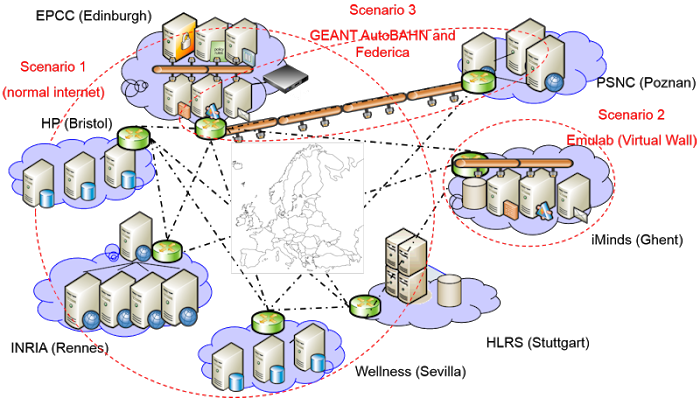
\includegraphics[width=0.85\textwidth]{statement/bonfire-testbeds.png}
\caption{BonFIRE testbeds.}
\label{fig:intr-bonfire-testbeds}
\end{center}
\end{figure}

The setup of the compute resources can be done by using contextualization variables in
order to provide important information for software applications in the virtual
machines.
This testbed also offers elasticity resources, that are dynamically created,
updated and destroyed according to the execution environment.

\begin{table}[H]
  \centering
  {\small
  


\begin{tabular}{p{0.2\textwidth}p{0.2\textwidth}p{0.2\textwidth}p{0.2\textwidth}}
  \tabheadformat
  \tabhead{Name}   &\tabhead{CPU cores} &\tabhead{Memory} & \tabhead{Features}\\
\hline
\textit{Lite}         & 0.5 & 256 MB & \\
\hline
\textit{Small}         & 1 & 1 GB & \\
\hline
\textit{Medium}        & 2 & 2 GB & \\
\hline
\textit{Large}          & 2 & 4 GB & \\
\hline
\textit{Large+}         & 2 & 4 GB & Higher CPU clock speed\\
\hline
\textit{Large-en}        & 4 & 4 GB & \\
\hline
\textit{Xlarge}        & 4 & 8 GB & \\
\hline
\textit{Xlarge+}        & 4 & 8 GB & Higher CPU clock speed\\
\hline
\textit{Custom}        & User defined & User defined &VCPU must be an integer \\
\hline
\end{tabular}


% Local variables:
%   coding: utf-8
%   ispell-local-dictionary: "castellano8"
%   TeX-master: "main.tex"
% End:

  }
  \caption{Instance types of BonFIRE.}
  \label{table:intro-instance-types}
\end{table}


\subsection{Federated Tools}
\label{subsec:federatedtools}
In the \emph{Fed4FIRE} project, some tools for deploying, controlling and
monitoring the experiments have been developed.
Some of these tools are used only by developers to deploy, to provision, to
make reservations and to discover resources~\cite{Fed4FIRE2014}. These tools are \emph{Flack, Omni
  and SFI}, which have a common interface named \emph{SFA}.

The experimenters utilize the tools for controlling the experiments. These tools
are described as follows:
\begin{itemize}
\item \emph{NEPI:} the Network Experimentation Programming Interface, is a
  life-cycle management tool for network experiments. It is developed in Python
  and it provides a high-level interface to describe experiments, to provision
  resources, to control experiments and to collect all the results of the
  experiment. To highlight that this implementation provides an important way to
  manage and to make a workflow for an experiment~\cite{INRIA2014}.
\item \emph{\ac{OMF6}:} is a generic framework that facilitates the definition and
  orchestration of the experiments. It can be used for controling the experiment
    through a distributed infrastructure based on \ac{XMPP} and an Aggregate Manager
  that manages all the information flows. It can be integrated with \acs{OML} for
  provisioning, control and collection of all the information about the experiment.
\item \emph{\acf{OML}:} this tool provides an \ac{API} to collect
  the status of any sensor or device. It implements a reporting protocol
  composed by a client and a collection server. On the client side,
  any application can be implemented using the \ac{OML} \ac{API} for collecting any
  information about the status of the devices concerning the experiment.
\end{itemize}


\section{Graphical User Interfaces}

A \ac{GUI} is a software that facilitates the human-machine interaction using images and graphic items. Normally, the interactions are produced
by user actions directly and these actions corresponds to events. The \ac{GUI} events
are usually produced by the mouse, touchpad, keyboard or nowadays, a
touchscreen. When an event is located, a specific action is performed
changing the interface itself, or creating, updating or deleting data or to
accomplish a specific proceeding.


\subsection{Frameworks}

There are lots of graphical user interface engines or frameworks available for
Python~\cite{Athanasias2014}. Because the project is developed in Python, the user interface was also
developed in Python. In addition, the searched engines are multiplatform. Finally, considering these criteria, some frameworks and
libraries  such as \emph{PyGUI, PyGtk, PyGame, PyQt, PyKDE and WxPython} were studied:

\begin{itemize}
\item \emph {PyGUI:} it is an \ac{API} for building graphical user interfaces
  easily. It can be used in any platform or
  operative system. Furthermore, it use  PyOpenGL libraries and it is distributed under \ac{GPL} v3.
\item \emph{PyGtk:} It is a library set of Python with which the programmer can
  develop  programs with a graphical user interface easily. It is multiplatform
  and it is distributed under \ac{LGPL} licence with few restrictions.
\item \emph{PyGame:} is a set of Python modules facilitates the creation of games and
  multimedia software such as graphical user interfaces. \emph{Pygame} is fully portable and
  runs on nearly every platform and operative system. This engine evolves
  funcionality of \ac{SDL} library, OpenGL and provides Blender integration. It is
  distributed under \ac{GPL} v3.
\item \emph{PyQt:} is a Python binding for Qt development. Qt is a
  cross-platform  and \ac{GUI} framework for  developing graphical user interfaces. Qt
  is distributed under \ac{GPL} v3 and \ac{LGPL} license. It is developed by Nokia and it
  permits the development of software for mobile, embedded platforms, desktop platforms
  and any operative system.
\item \emph{WxPython:} is a \ac{GUI} toolkit for Python that allows us to create
  robust, highly functional graphical user interfaces easily and simply. It is
  implemented in Python and it is distributed under \ac{GPL} v3 license.
\end{itemize}


\section{Database}
%http://196.29.172.66:8080/jspui/bitstream/123456789/1834/1/E174.pdf
Since computer manage the users information, humans had tried to sort these data
and collect it from machines effectively. For this purpose, the databases were
created. The databases are conceptual models to orderly store the information. Another step forward was the creation of the \ac{DBMS}. The \ac{DBMS}
is a software to manage the information contained into database to concentrate,
to arrange and to provide lots of mechanisms to manage the information contained
into database repository~\cite{Group2010}.

\subsection{DBMS}

In order to simulate the constellation of satellites for GEO-Cloud project, some
free \ac{DBMS} were studied. The most interesting are the following:
\begin{itemize}
%http://www.mysql.com/
\item \textbf{MySQL:} open source relational database management system developed by
  \emph{MySQL AB}. It is the most used database system in web applications. \emph{MySQL} provides triggers, cursors, sub-selects, stored
  procedures, an embedded database library and efficiently works with distributed systems. This \ac{DBMS} is multiplatform and it works in any
  operative system~\footnote{For more information, see \url{http://www.mysql.com/}}.
%https://www.monetdb.org/Home
\item \textbf{MonetDB:} open source column-oriented database management system
  developed by \emph{Centrum Wiskunde \& Informatica} in Netherlands. It offers
  high performance on complex queries in large databases combining tables with
  lots of columns and multi-million rows. This \ac{DBMS} is performed in data
  mining and geographic information systems~\footnote{For more information, see \url{https://www.monetdb.org/Home}}.
%http://www.postgresql.org.es/
\item \textbf{PostgreSQL:} \emph{PostgreSQL} is an object-oriented relational
  distributed database management system developed by \emph{PostgreSQL Global
    Development Team}. It is distributed under \ac{BSD} license. This database uses a
  client-server model based on multi-processing for granting system stability~\footnote{For more information, see \url{http://www.postgresql.org.es/}}.
\end{itemize}

\emph{MySQL} was selected in the project development because there are quite documentation and the
syntax is similar to \ac{SQL}.

\section{Distributed Systems}

Nowadays, most of applications need to obtain information from other sources
or to communicate with another hardware either other computers or
devices. As a
result, some programming paradigms like client-server, remote procedure call and
remote object invocation were born~\cite{Tanenbaum2008}.
\begin{itemize}
\item \textbf{Client-Server paradigm}~\\
This architecture is composed by two parts: the first one is the server
component and the second one is the client. The server is listening request from
clients and when an application comes the server decodes, processes it and
sends back the reply to the client.

\textbf{Remote Procedure Call}~\\
Remote Procedure Call uses the same principle as Client-Server but in a more
complex way. Basically, in remote procedure call paradigm, a client calls a
function as if it were a local function on the client machine, but this called
function is located in another machine which performs the function and returns
the results.

\textbf{Remote Object Invocation}~\\
This paradigm was born when the object-oriented programming paradigm was
developed. There are distributed objects and these objects are not
necessary fixed in a host. When a distributed-object is created, it is
bound to a set of machines as slave, so when a client application recovers that
object using a distributed-object registry or another one like that, the
provided operations by the distributed object can be remotely performed as if
it was a  operation call in applicant machine.
\end{itemize}

\subsection{Middleware}

For client-server paradigm there are not any middleware for developing
applications. Normally these applications are developed using the standard
oriented socket libraries.
For \ac{RPC} development, there are several implementations such as
\ac{SOAP}, \ac{CORBA}, UNIX \ac{RPC} and Pyro.

For Remote Object Invocation paradigm, there are several novel middlewares. The most used are
Hadoop and ZeroC \ac{ICE} and its features are as follows:

\subsubsection{Hadoop}
%http://hadoop.apache.org/
\emph{Hadoop}~\cite{Foundation2008} is a framework for developing  reliable and scalable
distributed applications. It is based on
the architecture used by \emph{Google} named ``MapReduce'' and other components
like \emph{Google File System}.
Some of its components are the following:
\begin{itemize}
\item \emph{Hadoop Common:} the common utilities for other Hadoop modules.
\item \emph{Hadoop Distributed File System:} distributed file system that
  provides high-throughput access.
\item \emph{Hadoop YARN:} a framework for job scheduling and resource management.
\item \emph{Hadoop MapReduce:} a YARN-based system for parallel processing of
  large data sets.
\end{itemize}
It is designed for scaling up thousands of machines. It
is maintained and distributed by \emph{Apache Software Foundation} under \ac{GPL} v.3
license.

\subsubsection{ZeroC ICE}
%http://www.zeroc.com/
\emph{ZeroC \ac{ICE}}, the internet communications engine, is a modern distributed computing
platform. It supports languages such as C++,Python, Java and Ruby among others.
It allows developers to create new powerful, efficient and simple applications
with minimal effort~\cite{ZeroC2013}.
The main features of this middleware are the following:

\begin{itemize}
\item It is a general-purpose distributed computing platform.
\item It uses a modern and flexible specification language.
\item Dynamic invocation and dispatch are supported.
\item Request Forwarding is provided.
\item Asynchronous and synchronous invocation and dispatch.
\item One-way, datagram and batched invocation are also supported.
\item Multi-threading software developments are fully thread-safe.
\item Several transport protocols can be used as \ac{TCP},\ac{SSL},\ac{UDP} and also \ac{IP}v4 and
  \ac{IP}v6 are supported.
\end{itemize}

\ac{ICE} provides the following services:
\begin{itemize}
\item \emph{IceGrid:} it is a service for large-scale grid computing applications.
\item \emph{IceStorm:} it is a sophisticated event distribution service.
\item \emph{Freeze:} it provides object persistence and the possibility to migrate
  these objects to a database.
\item \emph{Glacier2:} it is a firewall service.
\item \emph{IcePatch2:} it is a software and files distribution service.
\end{itemize}

\section{Software Design}

In this section, the software engineering knowledge and the software portability required by this project are studied. These areas are
described in the following subsections.

\subsection{Multiplatform source}

One of the main objectives of GEO-Cloud consists of the software portability. As
this project is an experiment, it has to be checked in any platform with any
operative system, so the developed source was written in Python. Among the huge variety of Python
interpreters, the used version in this project source was Python 2.7.

\emph{GNU/Linux} was the platform in which the development of all project files were
carried out. Besides the libraries distributed within Python, \emph{Paramiko}
Python library~\cite{Team2013} was used. This library implements \ac{SSH} protocol operations
for remotely managing and controlling machines. This library is distributed
under \ac{GPL} v3.
http://www.lag.net/paramiko/

\subsection{Software Development Life Cycles}

Historically, the software
was developed without any methodology, so there were lots of bugs in the
code. As a result, programs did not work correctly or they were inefficient or
inclusive, they stopped unexpectedly. Then the saviour programmer tried to solve
the trouble wasting lot of time. Thus, the software development was very
expensive~\cite{Garcia2013}.
At present, the software development is guided by life cycles. In this cycles,
stages such as planning, designing, implementation, testing, documenting, deployment
and maintenance are basics for software development. Depending on how these
stages are done, there are several life cycles. Among others, the most important and
more used are the following:

\begin{itemize}
\item \emph{Waterfall model:} strict model in which the developers have to
  follow the following stages in order: analisys, design, implementation, testing, deployment and maintenance.
\item \emph{Spiral model:} this life cycle combines the waterfall model and rapid
  prototyping.
\item \emph{Iterative and incremental cycle:} it is based on the development of small but
  ever-larger portions of a software. During software development, several
  iterations may be in progress at the same time. Using this cycle, the
  end-users can check the no-ended product for updating requirements or for giving feedback
  to end-user.
\item \emph{Agile development:} this model is very used nowadays. Its principles
  are the iterative development and the incorporation of continuous feedback and
  staging iterations.
\end{itemize}

\subsection{Design Patterns}

The software programming patterns that were studied in the development of
GEO-Cloud experiment are the following:
\begin{itemize}
\item Singleton: only a single instance of a class can exist.
\item Composite: a tree structure of simple and composite objects.
\item Proxy: an object that represents another one.
\end{itemize}

\subsection{Testing}

While the GEO-Cloud software was being developed, the testing process was
done. The testing was done as follows: hand testing and test-case oriented
testing. In test-case oriented testing, sundry testing frameworks were studied.
The selected framework for testing in Python was \emph{UnitTest} and its
extension \emph{Nose}. It is included in Python standard library, it is easy to use
and it has lots of plugins~\cite{Foundation2014a}.

The developed test-cases were black-box essentially. Some white box test-cases
were developed but the code coverage was not thorough.
